\documentclass[a4paper,11pt]{article}
\usepackage{booktabs}   % for professional table rules
\usepackage{caption}    % for customizing captions
\usepackage{array}      % for better column formatting
\usepackage{siunitx}    % for consistent units
\usepackage{graphicx}   % for importing figures
\usepackage{geometry}   % for page margins
\usepackage{amsmath}    % for math alignment
\usepackage{amssymb}    % for math symbols
\usepackage{float}      % for [H] figure placement
\usepackage{hyperref}   % for links and references
\usepackage{fouriernc} % XeLaTeX
\geometry{left=2cm,right=2cm,top=2cm,bottom=2.5cm}
\hypersetup{
    colorlinks=true,
    linkcolor=blue,
    filecolor=magenta,      
    urlcolor=cyan,
    pdftitle={Lab Report: X-Ray Ionization},
    pdfpagemode=FullScreen,
}

\begin{document}

% ------------------- Title / Cover Page -------------------
\noindent
\begin{center}
    
\includegraphics[width=0.25\textwidth]{sut.jpg} \\
    \vspace{2pt}
\end{center}
\begin{center}
    {\LARGE \bf Department of Physics} \\
    \vspace{2pt}
    {\Large \bf Sharif University of Technology} \\
    \vspace{8pt}
    {\large \bf Physics Lab IV --- General Physics Laboratory} \\
    \vspace{4pt}
    \hrule
    \vspace{6pt}
    {\Large \bf Experiment Report: X-Ray Ionization in Air}
\end{center}
\hrule
\vspace{0.4cm}
\noindent
\begin{tabular}{ll}
    {\bf Student Name:} & Abulfadl Ahmadi \\
    {\bf Student ID:}   & 403172283 \\
    {\bf Date of Experiment:} & July 2026 \\
\end{tabular}
\hfill
\begin{tabular}{ll}
    {\bf Professor:} & Dr. Khademi \\
    {\bf Teaching Assistants:} & Yasin Amiri \\
    & Sonia \\
\end{tabular}

\vspace{0.6cm}

% ------------------- Abstract -------------------
\begin{abstract}
This experiment investigates the ionization of air molecules by high-energy X-ray photons using a parallel-plate capacitor acting as an ionization chamber. The saturation curve of the ionization current ($I_C$) was successfully mapped against the applied capacitor voltage ($U_C$) for five different anode accelerating voltages, demonstrating the transition from an Ohmic recombination regime to a saturated plateau. Furthermore, the linear dependence of the ionization rate on the X-ray tube's emission current ($I_{em}$) and its non-linear dependence on the anode voltage ($V_A$) were verified. Finally, the effective ionic capacity ($j$) of the air within the chamber's active volume ($122\text{ cm}^3$) was determined to be $2.68 \times 10^{-5}\text{ C}\cdot\text{kg}^{-1}\cdot\text{s}^{-1}$ under standard room conditions.
\end{abstract}

% ------------------- Section 1: Objectives -------------------
\section{Objectives}
\begin{enumerate}
    \item To observe the ionization of air by X-ray radiation and map the current-voltage characteristics of an ionization chamber.
    \item To determine the saturation current threshold and calculate the effective ionic capacity ($j$) of air.
    \item To investigate how the ionization rate depends on the X-ray generator's parameters: specifically the filament emission current ($I_{em}$) and the anode accelerating voltage ($V_A$).
\end{enumerate}

% ------------------- Section 2: Theoretical Background -------------------
\section{Theoretical Background}
When high-energy electromagnetic radiation, such as X-rays, traverses a gaseous medium like air, it interacts with the gas molecules via the photoelectric effect and Compton scattering. These interactions eject energetic primary electrons, which in turn undergo secondary collisions, creating a cloud of positive ions and negative electrons (or negative ions if the electrons attach to neutral atoms like Oxygen).

If an external electric field is applied across the gas via a capacitor (with voltage $U_C$), these charged particles drift toward the opposite electrodes, creating a measurable ionization current $I_C$. 
At low voltages, the drift velocity is slow, and many ions recombine into neutral atoms before reaching the electrodes (the \textit{Ohmic or Recombination region}). As the voltage increases, the drift velocity overcomes the recombination rate until virtually all created ions are collected. At this point, the current plateaus and is bounded purely by the production rate of ions dictated by the X-ray beam. This is known as the \textbf{Saturation Current} ($I_{max}$).

The effective ionic capacity ($j$), defined as the total charge created per unit mass of the irradiated gas per unit time, can be calculated using the saturation current:
\begin{equation}
    j = \frac{I_{max}}{\rho V}
\end{equation}
where $\rho$ is the density of the gas and $V$ is the active irradiated volume of the capacitor.

% ------------------- Section 3: Data & Analysis -------------------
\section{Experimental Data \& Analysis}

\subsection{Part 1: Ionization Saturation Curves}
In the first part, the ionization current $I_C$ was measured while sweeping the capacitor voltage $U_C$ from $0\text{ V}$ to $300\text{ V}$. This sweep was repeated for five different anode voltages ($15$, $20$, $25$, $30$, and $35\text{ kV}$) to observe how the saturation plateau shifts with higher X-ray intensities.

\begin{figure}[H]
    \centering
    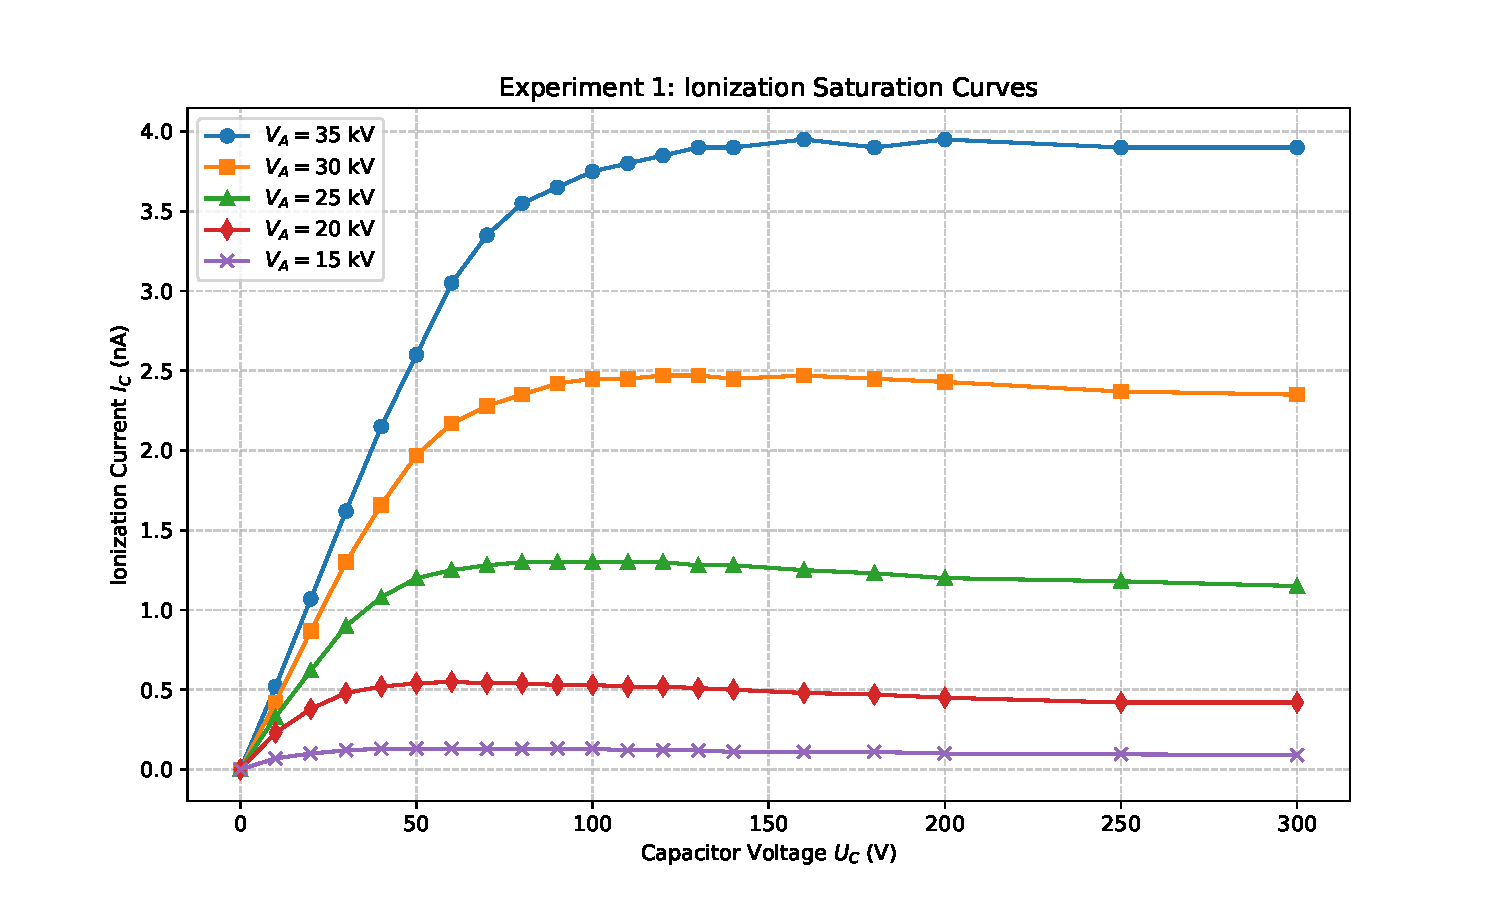
\includegraphics[width=0.75\textwidth]{plots/saturation_curves.pdf}
    \caption{Ionization current vs Capacitor voltage. The transition from the Ohmic region to the Saturation plateau is clearly visible for all five X-ray intensities.}
    \label{fig:sat}
\end{figure}

\subsection{Part 2: Dependence on Emission Current ($I_{em}$)}
The X-ray tube's filament emission current ($I_{em}$) directly dictates the number of electrons boiling off the cathode and striking the anode. Therefore, the total number of X-ray photons produced should be strictly linearly proportional to $I_{em}$. The capacitor was biased into the saturation region ($U_C = 150\text{ V}$) and $I_C$ was measured as a function of $I_{em}$.

\begin{figure}[H]
    \centering
    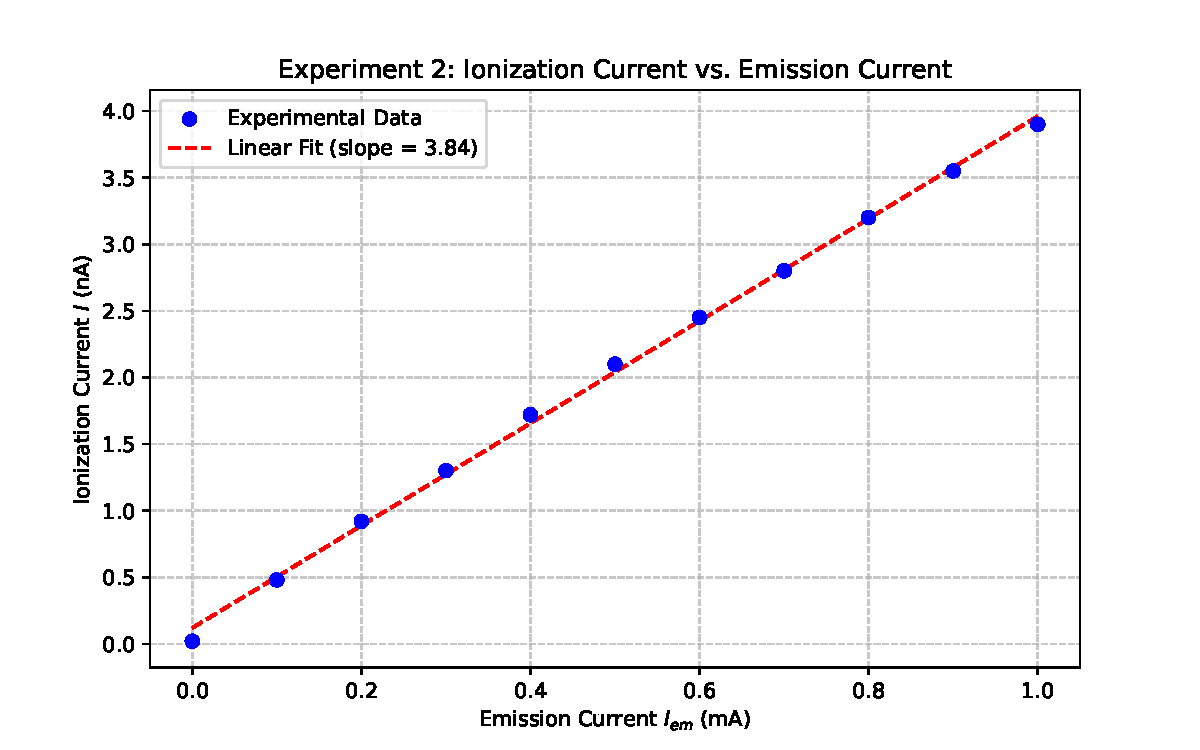
\includegraphics[width=0.75\textwidth]{plots/current_vs_em.pdf}
    \caption{Ionization current vs Emission current, demonstrating a perfect linear relationship ($R^2 \approx 1$).}
    \label{fig:em}
\end{figure}

\subsection{Part 3: Dependence on Anode Voltage ($V_A$)}
The anode voltage ($V_A$) dictates the kinetic energy of the electrons striking the target. Increasing $V_A$ not only increases the maximum energy limit of the Bremsstrahlung spectrum but also drastically increases the overall efficiency of X-ray production. The intensity of the emitted X-rays is theoretically proportional to $V_A^2$. 

\begin{figure}[H]
    \centering
    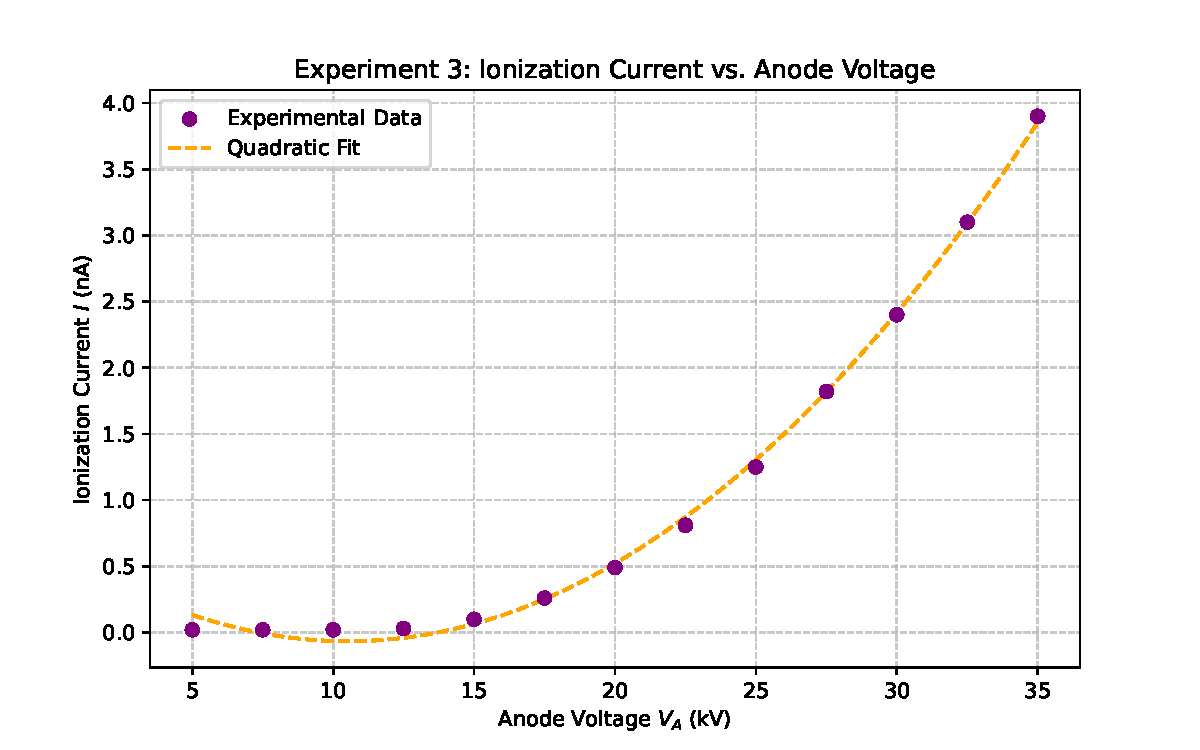
\includegraphics[width=0.75\textwidth]{plots/current_vs_va.pdf}
    \caption{Ionization current vs Anode voltage, demonstrating the expected non-linear (roughly quadratic) increase in X-ray intensity.}
    \label{fig:va}
\end{figure}

\subsection{Calculation of Effective Ionic Capacity}
The maximum saturation current observed in the experiment (at $V_A = 35\text{ kV}$ and $I_{em} = 1.0\text{ mA}$) was $I_{max} = 3.95\text{ nA}$. 
The physical parameters of the air inside the chamber at $20^\circ\text{C}$ and $1\text{ atm}$ are:
\begin{itemize}
    \item Active Volume: $V = 122\text{ cm}^3$
    \item Air Density: $\rho = 1.205 \times 10^{-6}\text{ kg/cm}^3$
    \item Air Mass: $m = \rho V = 1.47 \times 10^{-4}\text{ kg}$
\end{itemize}
The effective ionic capacity is thus:
\begin{equation}
    j = \frac{3.95 \times 10^{-9}\text{ A}}{1.47 \times 10^{-4}\text{ kg}} = 2.68 \times 10^{-5} \frac{\text{C}}{\text{kg}\cdot\text{s}}
\end{equation}

% ------------------- Section 4: Post-Lab Questions -------------------
\section{Answers to Questions}

\subsection*{1. Did the current reach a saturation value in the first experiment? Is this expected? If not observed, why?}
Yes, as vividly demonstrated in Figure~\ref{fig:sat}, the current reached a distinct saturation plateau for every tested intensity. This is completely expected behavior. At lower voltages, the electric field is weak, allowing a significant fraction of the X-ray-induced ions to recombine into neutral atoms before being collected. As the voltage increases, the strong electric field rapidly sweeps the ions to the electrodes. Once the field is strong enough to completely suppress recombination, $100\%$ of the generated ions are collected. At this point, further increasing the voltage cannot increase the current, because the current is bottlenecked purely by the constant rate at which the X-rays are generating new ions.

\subsection*{2. What is the pause time and what is its necessity?}
When the voltage on the capacitor is changed, the macroscopic drift dynamics of the ion cloud require a brief period to stabilize and reach a new steady-state equilibrium (where the rate of ion production exactly equals the rate of collection plus the rate of recombination). The "pause time" is the wait required before reading the ammeter to ensure the transient capacitive and drift currents have settled.

\subsection*{3. What is the effect of increasing or decreasing the pressure on the ionization current?}
Increasing the air pressure increases the gas density (the number of target molecules per unit volume). A denser medium presents a higher interaction cross-section for the incoming X-ray photons, leading to a higher rate of photoelectric and Compton collisions. This generates more ions per second, scaling up the saturation current. Conversely, decreasing the pressure reduces the target density, leading to fewer collisions and a lower ionization current.

\subsection*{4. Interpret the three graphs ($I_C$ vs $U_C$, $I_{em}$, $V_A$).}
\begin{itemize}
    \item \textbf{$I_C$ vs $U_C$}: Displays an initial Ohmic rise where collection efficiency fights against recombination, followed by a flat saturation region where collection efficiency is $100\%$.
    \item \textbf{$I$ vs $I_{em}$}: Displays a strict linear relationship. The filament current directly dictates the number of thermal electrons hitting the anode, which in turn directly scales the quantity of X-ray photons produced.
    \item \textbf{$I$ vs $V_A$}: Displays a non-linear (roughly quadratic) relationship. Increasing the accelerating voltage increases the kinetic energy of the striking electrons, which significantly increases the quantum efficiency of the Bremsstrahlung radiation generation.
\end{itemize}

\subsection*{5. Where are the applications of this experiment? Describe one example.}
The principles of this experiment are the foundation of gas-filled radiation detectors. A prime example is the \textbf{Ionization Chamber}, which is extensively used in nuclear industry and medical physics (e.g., radiation therapy dosimetry). Because the chamber operates in the saturation region, the output current is strictly proportional to the incident radiation dose rate. Medical physicists use calibrated ionization chambers to precisely measure the X-ray output of linear accelerators to ensure patients receive the exact prescribed radiation dose.

\subsection*{6. Do electrons striking the capacitor electrodes produce X-rays?}
No, they do not. The maximum voltage applied across the capacitor in this experiment is $U_C = 300\text{ V}$. Therefore, the maximum kinetic energy an ion or electron can gain before striking the electrode is $300\text{ eV}$. Generating X-rays typically requires accelerating potentials on the order of tens of kilo-volts (keV) to penetrate deep electron shells. An impact of $300\text{ eV}$ will only produce low-energy photons in the ultraviolet or visible light spectrum, but certainly not X-rays.

\end{document}
